\begin{figure}[htb]
\centering
\begin{subfigure}[b]{.45\columnwidth}
\centering
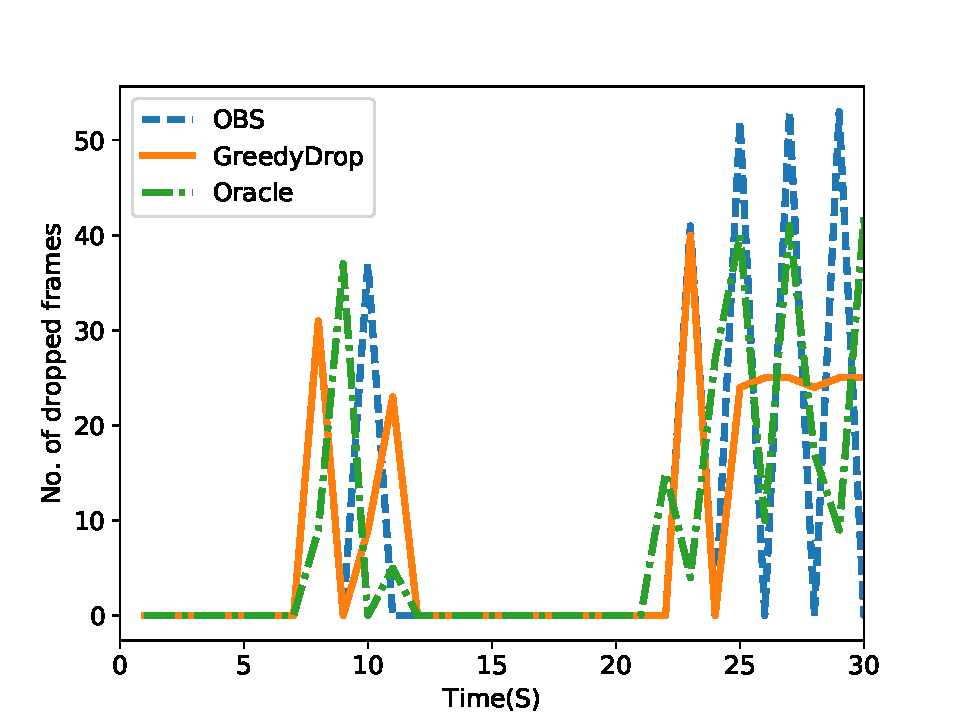
\includegraphics[width=\linewidth]{fig/drop-buffer.pdf}
\caption{No. of frame drop}
\label{fig:drop-buffer}\mylabel{fig:drop-buffer}
\end{subfigure}
\begin{subfigure}[b]{.45\columnwidth}
\centering
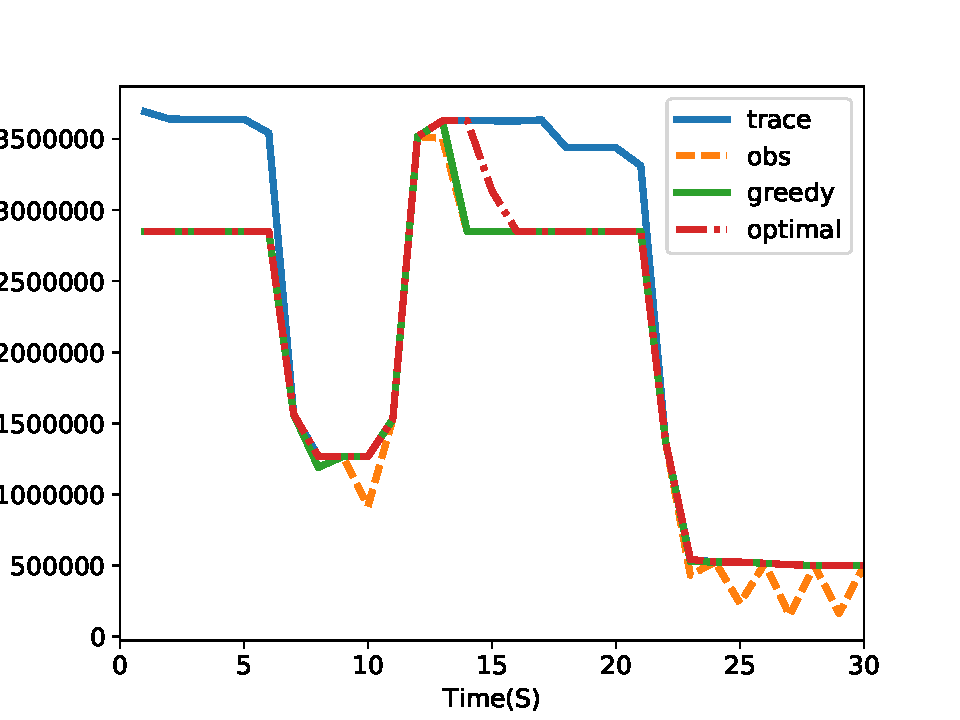
\includegraphics[width=\linewidth]{fig/drop-bandwidth.pdf}
\caption{Real-time throughput}
\label{fig:drop-bandwidth}\mylabel{fig:drop-bandwidth}
\end{subfigure}
\caption{Comparison of different frame drop strategy}
\vspace{-0.15in}
\end{figure} 